\documentclass[10pt]{article}
\usepackage[T1]{fontenc}
\usepackage[letterpaper,landscape,margin=0.22in]{geometry}
\usepackage{tgbonum}
\usepackage[dvipsnames]{xcolor}
\usepackage{tikz}
\usetikzlibrary{calc}

\pagestyle{empty}
\setlength{\parindent}{0pt}

\definecolor{BoardInk}{HTML}{17212B}
\definecolor{BoardGray}{HTML}{E9EDF0}
\definecolor{BoardLight}{HTML}{F7F8F9}
\definecolor{TerranBlue}{HTML}{167DA4}
\definecolor{TerranPale}{HTML}{DDEFF5}
\definecolor{ImperialRed}{HTML}{A23B3B}
\definecolor{ImperialPale}{HTML}{F4E1E1}
\definecolor{RangeGold}{HTML}{D2A93B}

\begin{document}
\centering
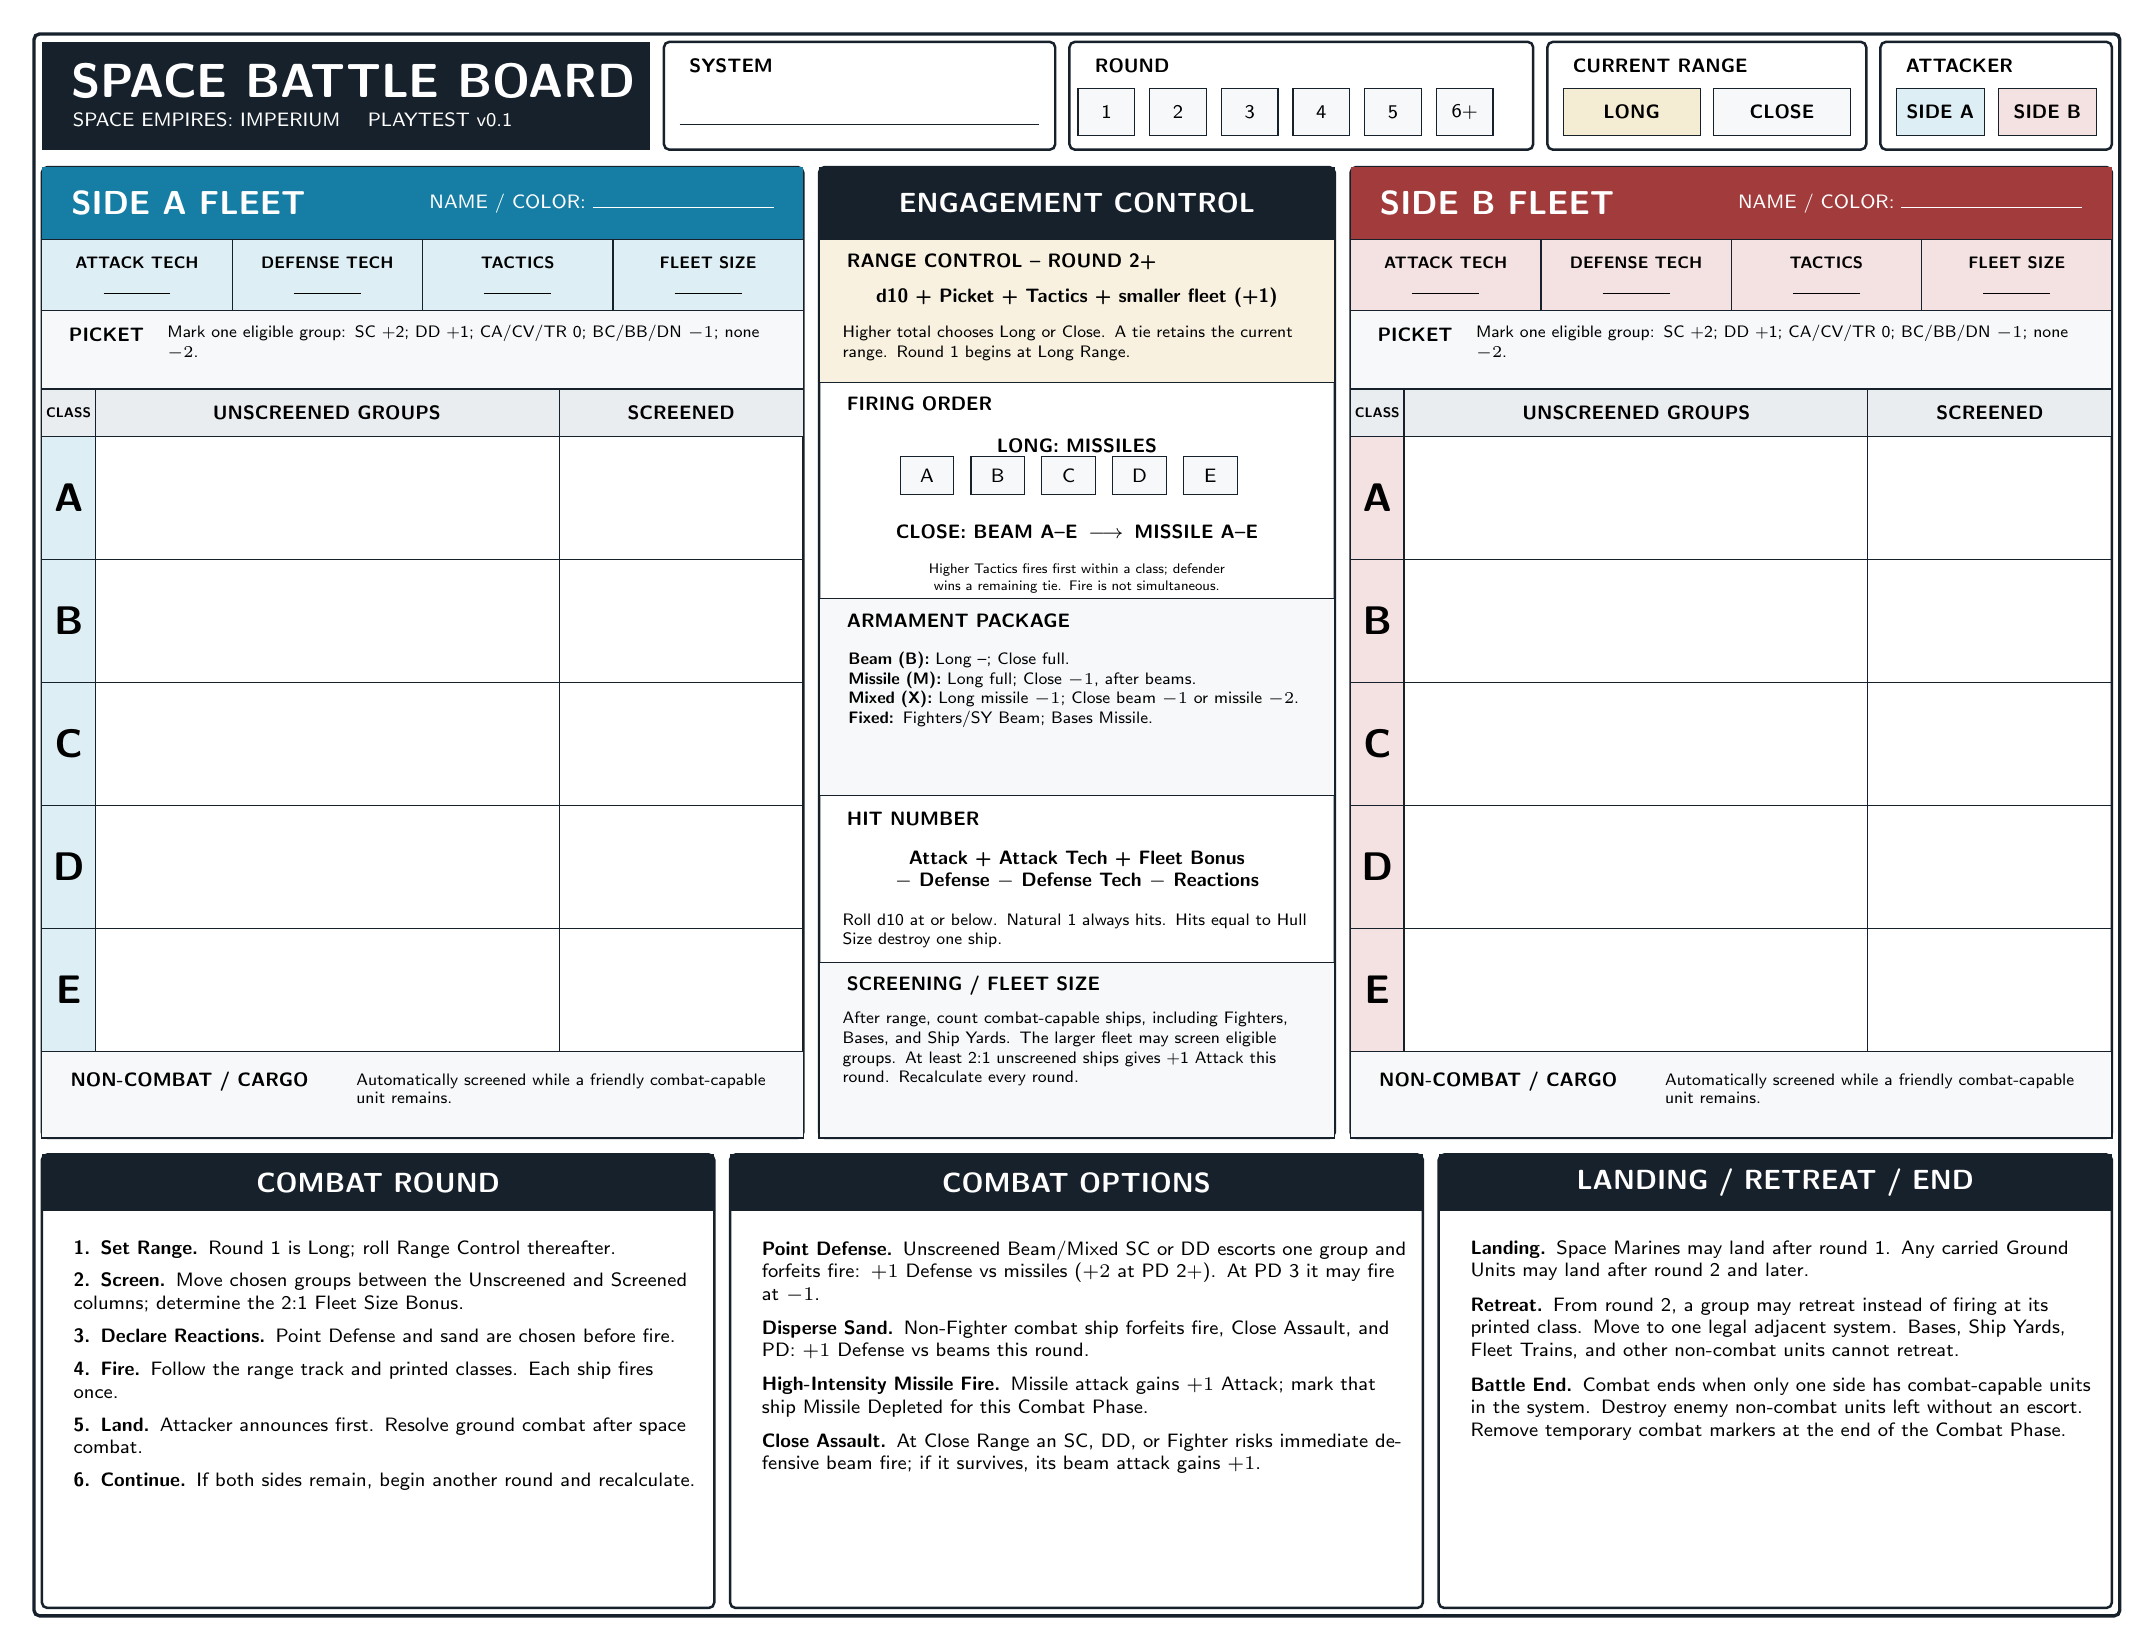
\begin{tikzpicture}[
  x=1cm,y=1cm,
  outer/.style={draw=BoardInk,line width=0.9pt,rounded corners=2pt},
  rule/.style={draw=BoardInk,line width=0.45pt},
  heading/.style={font=\bfseries\sffamily},
  label/.style={font=\bfseries\sffamily\scriptsize},
  note/.style={font=\sffamily\fontsize{6.4}{7.2}\selectfont,align=left},
  micronote/.style={font=\sffamily\fontsize{5.8}{6.5}\selectfont,align=left},
  bottomnote/.style={font=\sffamily\fontsize{7}{8.2}\selectfont,align=left},
  centertext/.style={font=\sffamily\scriptsize,align=center}
]
  \path[use as bounding box] (0,0) rectangle (26.65,20.25);
  \draw[outer,line width=1.2pt] (0.08,0.08) rectangle (26.57,20.17);

  % Header
  \fill[BoardInk] (0.18,18.70) rectangle (7.90,20.07);
  \node[anchor=west,text=white,font=\bfseries\sffamily\LARGE]
    at (0.43,19.58) {SPACE BATTLE BOARD};
  \node[anchor=west,text=white,font=\sffamily\scriptsize]
    at (0.45,19.08) {SPACE EMPIRES: IMPERIUM \quad PLAYTEST v0.1};

  \draw[outer] (8.08,18.70) rectangle (13.05,20.07);
  \node[label,anchor=west] at (8.28,19.76) {SYSTEM};
  \draw[rule] (8.28,19.02) -- (12.84,19.02);

  \draw[outer] (13.23,18.70) rectangle (19.12,20.07);
  \node[label,anchor=west] at (13.43,19.76) {ROUND};
  \foreach \n [count=\i from 0,evaluate=\i as \x using 13.34+0.91*\i]
    in {1,2,3,4,5,6+} {
    \draw[rule,fill=BoardLight] (\x,18.88) rectangle +(0.72,0.60);
    \node[centertext] at ($(\x,18.88)+(0.36,0.30)$) {\n};
  }

  \draw[outer] (19.30,18.70) rectangle (23.35,20.07);
  \node[label,anchor=west] at (19.50,19.76) {CURRENT RANGE};
  \draw[rule,fill=RangeGold!22] (19.50,18.88) rectangle (21.24,19.48);
  \draw[rule,fill=BoardLight] (21.41,18.88) rectangle (23.15,19.48);
  \node[centertext,font=\bfseries\sffamily\scriptsize] at (20.37,19.18) {LONG};
  \node[centertext,font=\bfseries\sffamily\scriptsize] at (22.28,19.18) {CLOSE};

  \draw[outer] (23.53,18.70) rectangle (26.47,20.07);
  \node[label,anchor=west] at (23.73,19.76) {ATTACKER};
  \draw[rule,fill=TerranPale] (23.73,18.88) rectangle (24.85,19.48);
  \draw[rule,fill=ImperialPale] (25.03,18.88) rectangle (26.27,19.48);
  \node[centertext,font=\bfseries\sffamily\scriptsize] at (24.29,19.18) {SIDE A};
  \node[centertext,font=\bfseries\sffamily\scriptsize] at (25.65,19.18) {SIDE B};

  % Side A fleet panel
  \draw[outer] (0.18,6.15) rectangle (9.85,18.48);
  \fill[TerranBlue] (0.18,17.56) rectangle (9.85,18.48);
  \node[anchor=west,text=white,font=\bfseries\sffamily\large]
    at (0.43,18.02) {SIDE A FLEET};
  \node[anchor=east,text=white,font=\sffamily\scriptsize]
    at (9.60,18.02) {NAME / COLOR: \rule{2.3cm}{0.35pt}};

  \foreach \i/\txt in {0/ATTACK TECH,1/DEFENSE TECH,2/TACTICS,3/FLEET SIZE} {
    \pgfmathsetmacro{\xa}{0.18+2.4175*\i}
    \pgfmathsetmacro{\xb}{0.18+2.4175*(\i+1)}
    \draw[rule,fill=TerranPale] (\xa,16.66) rectangle (\xb,17.56);
    \node[centertext,font=\bfseries\sffamily\fontsize{6.2}{7}\selectfont]
      at ({(\xa+\xb)/2},17.26) {\txt};
    \node[centertext] at ({(\xa+\xb)/2},16.88) {\rule{0.85cm}{0.3pt}};
  }

  \draw[rule,fill=BoardLight] (0.18,15.66) rectangle (9.85,16.66);
  \node[label,anchor=west] at (0.40,16.35) {PICKET};
  \node[note,anchor=west,text width=7.8cm] at (1.65,16.25)
    {Mark one eligible group: SC +2; DD +1; CA/CV/TR 0; BC/BB/DN $-1$; none $-2$.};

  \fill[BoardGray] (0.18,15.06) rectangle (9.85,15.66);
  \draw[rule] (0.18,15.06) rectangle (9.85,15.66);
  \draw[rule] (0.86,15.06) -- (0.86,15.66);
  \draw[rule] (6.75,15.06) -- (6.75,15.66);
  \node[font=\bfseries\sffamily\fontsize{5.5}{6}\selectfont] at (0.52,15.36) {CLASS};
  \node[label] at (3.80,15.36) {UNSCREENED GROUPS};
  \node[label] at (8.30,15.36) {SCREENED};

  \foreach \lab/\yb/\yt in {A/13.498/15.06,B/11.936/13.498,C/10.374/11.936,D/8.812/10.374,E/7.25/8.812} {
    \draw[rule] (0.18,\yb) rectangle (9.85,\yt);
    \draw[rule,fill=TerranPale] (0.18,\yb) rectangle (0.86,\yt);
    \draw[rule] (6.75,\yb) -- (6.75,\yt);
    \node[font=\bfseries\sffamily\Large] at (0.52,{(\yb+\yt)/2}) {\lab};
  }
  \draw[rule,fill=BoardLight] (0.18,6.15) rectangle (9.85,7.25);
  \node[label,anchor=west] at (0.42,6.87) {NON-COMBAT / CARGO};
  \node[micronote,anchor=west,text width=5.3cm] at (4.05,6.78)
    {Automatically screened while a friendly combat-capable unit remains.};

  % Side B fleet panel
  \draw[outer] (16.80,6.15) rectangle (26.47,18.48);
  \fill[ImperialRed] (16.80,17.56) rectangle (26.47,18.48);
  \node[anchor=west,text=white,font=\bfseries\sffamily\large]
    at (17.05,18.02) {SIDE B FLEET};
  \node[anchor=east,text=white,font=\sffamily\scriptsize]
    at (26.22,18.02) {NAME / COLOR: \rule{2.3cm}{0.35pt}};

  \foreach \i/\txt in {0/ATTACK TECH,1/DEFENSE TECH,2/TACTICS,3/FLEET SIZE} {
    \pgfmathsetmacro{\xa}{16.80+2.4175*\i}
    \pgfmathsetmacro{\xb}{16.80+2.4175*(\i+1)}
    \draw[rule,fill=ImperialPale] (\xa,16.66) rectangle (\xb,17.56);
    \node[centertext,font=\bfseries\sffamily\fontsize{6.2}{7}\selectfont]
      at ({(\xa+\xb)/2},17.26) {\txt};
    \node[centertext] at ({(\xa+\xb)/2},16.88) {\rule{0.85cm}{0.3pt}};
  }

  \draw[rule,fill=BoardLight] (16.80,15.66) rectangle (26.47,16.66);
  \node[label,anchor=west] at (17.02,16.35) {PICKET};
  \node[note,anchor=west,text width=7.8cm] at (18.27,16.25)
    {Mark one eligible group: SC +2; DD +1; CA/CV/TR 0; BC/BB/DN $-1$; none $-2$.};

  \fill[BoardGray] (16.80,15.06) rectangle (26.47,15.66);
  \draw[rule] (16.80,15.06) rectangle (26.47,15.66);
  \draw[rule] (17.48,15.06) -- (17.48,15.66);
  \draw[rule] (23.37,15.06) -- (23.37,15.66);
  \node[font=\bfseries\sffamily\fontsize{5.5}{6}\selectfont] at (17.14,15.36) {CLASS};
  \node[label] at (20.43,15.36) {UNSCREENED GROUPS};
  \node[label] at (24.92,15.36) {SCREENED};

  \foreach \lab/\yb/\yt in {A/13.498/15.06,B/11.936/13.498,C/10.374/11.936,D/8.812/10.374,E/7.25/8.812} {
    \draw[rule] (16.80,\yb) rectangle (26.47,\yt);
    \draw[rule,fill=ImperialPale] (16.80,\yb) rectangle (17.48,\yt);
    \draw[rule] (23.37,\yb) -- (23.37,\yt);
    \node[font=\bfseries\sffamily\Large] at (17.14,{(\yb+\yt)/2}) {\lab};
  }
  \draw[rule,fill=BoardLight] (16.80,6.15) rectangle (26.47,7.25);
  \node[label,anchor=west] at (17.04,6.87) {NON-COMBAT / CARGO};
  \node[micronote,anchor=west,text width=5.3cm] at (20.67,6.78)
    {Automatically screened while a friendly combat-capable unit remains.};

  % Central engagement-control panel
  \draw[outer] (10.05,6.15) rectangle (16.60,18.48);
  \fill[BoardInk] (10.05,17.56) rectangle (16.60,18.48);
  \node[text=white,font=\bfseries\sffamily\normalsize] at (13.325,18.02)
    {ENGAGEMENT CONTROL};

  \draw[rule,fill=RangeGold!16] (10.05,15.74) rectangle (16.60,17.56);
  \node[label,anchor=west] at (10.28,17.27) {RANGE CONTROL -- ROUND 2+};
  \node[centertext,font=\bfseries\sffamily\scriptsize] at (13.325,16.82)
    {d10 + Picket + Tactics + smaller fleet (+1)};
  \node[note,text width=5.95cm] at (13.325,16.24)
    {Higher total chooses Long or Close. A tie retains the current range. Round 1 begins at Long Range.};

  \draw[rule] (10.05,13.00) rectangle (16.60,15.74);
  \node[label,anchor=west] at (10.28,15.47) {FIRING ORDER};
  \node[centertext,font=\bfseries\sffamily\scriptsize] at (13.325,14.94)
    {LONG: MISSILES};
  \foreach \lab [count=\i from 0] in {A,B,C,D,E} {
    \draw[rule,fill=BoardLight] ({11.08+0.90*\i},14.32) rectangle +(0.68,0.48);
    \node[centertext] at ({11.42+0.90*\i},14.56) {\lab};
  }
  \node[centertext,font=\bfseries\sffamily\scriptsize] at (13.325,13.85)
    {CLOSE: BEAM A--E \,$\longrightarrow$\, MISSILE A--E};
  \node[font=\sffamily\fontsize{5.5}{6.1}\selectfont,align=center,
    text width=5.95cm] at (13.325,13.25)
    {Higher Tactics fires first within a class; defender wins a remaining tie. Fire is not simultaneous.};

  \draw[rule,fill=BoardLight] (10.05,10.50) rectangle (16.60,13.00);
  \node[label,anchor=west] at (10.28,12.72) {ARMAMENT PACKAGE};
  \node[note,anchor=north west,text width=5.95cm] at (10.30,12.45) {
    \textbf{Beam (B):} Long --; Close full.\\
    \textbf{Missile (M):} Long full; Close $-1$, after beams.\\
    \textbf{Mixed (X):} Long missile $-1$; Close beam $-1$ or missile $-2$.\\
    \textbf{Fixed:} Fighters/SY Beam; Bases Missile.};

  \draw[rule] (10.05,8.38) rectangle (16.60,10.50);
  \node[label,anchor=west] at (10.28,10.20) {HIT NUMBER};
  \node[centertext,font=\bfseries\sffamily\fontsize{7}{8}\selectfont,
    text width=5.9cm] at (13.325,9.55)
    {Attack + Attack Tech + Fleet Bonus\\
     $-$ Defense $-$ Defense Tech $-$ Reactions};
  \node[note,text width=5.95cm] at (13.325,8.78)
    {Roll d10 at or below. Natural 1 always hits. Hits equal to Hull Size destroy one ship.};

  \draw[rule,fill=BoardLight] (10.05,6.15) rectangle (16.60,8.38);
  \node[label,anchor=west] at (10.28,8.08) {SCREENING / FLEET SIZE};
  \node[note,text width=5.95cm] at (13.325,7.28)
    {After range, count combat-capable ships, including Fighters, Bases, and Ship Yards. The larger fleet may screen eligible groups. At least 2:1 unscreened ships gives +1 Attack this round. Recalculate every round.};

  % Bottom reference panels
  \draw[outer] (0.18,0.18) rectangle (8.72,5.94);
  \fill[BoardInk] (0.18,5.22) rectangle (8.72,5.94);
  \node[text=white,font=\bfseries\sffamily\normalsize] at (4.45,5.58)
    {COMBAT ROUND};
  \node[bottomnote,anchor=north west,text width=8.0cm] at (0.46,4.97) {
    \textbf{1. Set Range.} Round 1 is Long; roll Range Control thereafter.\\[1.3mm]
    \textbf{2. Screen.} Move chosen groups between the Unscreened and Screened columns; determine the 2:1 Fleet Size Bonus.\\[1.3mm]
    \textbf{3. Declare Reactions.} Point Defense and sand are chosen before fire.\\[1.3mm]
    \textbf{4. Fire.} Follow the range track and printed classes. Each ship fires once.\\[1.3mm]
    \textbf{5. Land.} Attacker announces first. Resolve ground combat after space combat.\\[1.3mm]
    \textbf{6. Continue.} If both sides remain, begin another round and recalculate.};

  \draw[outer] (8.92,0.18) rectangle (17.72,5.94);
  \fill[BoardInk] (8.92,5.22) rectangle (17.72,5.94);
  \node[text=white,font=\bfseries\sffamily\normalsize] at (13.32,5.58)
    {COMBAT OPTIONS};
  \node[bottomnote,anchor=north west,text width=8.25cm] at (9.20,4.97) {
    \textbf{Point Defense.} Unscreened Beam/Mixed SC or DD escorts one group and forfeits fire: $+1$ Defense vs missiles ($+2$ at PD 2+). At PD 3 it may fire at $-1$.\\[1.4mm]
    \textbf{Disperse Sand.} Non-Fighter combat ship forfeits fire, Close Assault, and PD: $+1$ Defense vs beams this round.\\[1.4mm]
    \textbf{High-Intensity Missile Fire.} Missile attack gains $+1$ Attack; mark that ship Missile Depleted for this Combat Phase.\\[1.4mm]
    \textbf{Close Assault.} At Close Range an SC, DD, or Fighter risks immediate defensive beam fire; if it survives, its beam attack gains $+1$.};

  \draw[outer] (17.92,0.18) rectangle (26.47,5.94);
  \fill[BoardInk] (17.92,5.22) rectangle (26.47,5.94);
  \node[text=white,font=\bfseries\sffamily\normalsize] at (22.195,5.58)
    {LANDING / RETREAT / END};
  \node[bottomnote,anchor=north west,text width=8.0cm] at (18.20,4.97) {
    \textbf{Landing.} Space Marines may land after round 1. Any carried Ground Units may land after round 2 and later.\\[1.5mm]
    \textbf{Retreat.} From round 2, a group may retreat instead of firing at its printed class. Move to one legal adjacent system. Bases, Ship Yards, Fleet Trains, and other non-combat units cannot retreat.\\[1.5mm]
    \textbf{Battle End.} Combat ends when only one side has combat-capable units in the system. Destroy enemy non-combat units left without an escort. Remove temporary combat markers at the end of the Combat Phase.};
\end{tikzpicture}
\end{document}
